\subsection{Formationen}
Zur Bewegung durch das Gelände verwendet man Formationen, welche der sich bewegenden Gruppe Vor- und Nachteile bieten. Sie sollten jederzeit dem Gelände sowie erwarteten oder bekannten Feindkräften angepasst werden. Die Formationen welche im TTT Verwendung finden sind der \textit{Stack}, die \textit{Kolonne} und die \textit{Schützenkette}. 

\subsubsection{Der Stack}
Der Stack ist die Sammelformation vor dem Abmarsch und als Bewegungsformation beim Einstieg in Fahrzeuge. Zudem dient er als Formation für den direkten Zugriff in Räume (siehe dazu CQB \autoref{CQB}). Grundsätzlich wird der Stack in den klassischen (engen) <<Stack>> und <<Stack weit>> unterteilt. Beim <<Stack weit>> werden die Abstände lediglich erweitert.\\
\begin{figure}[!htb]
	\centering
	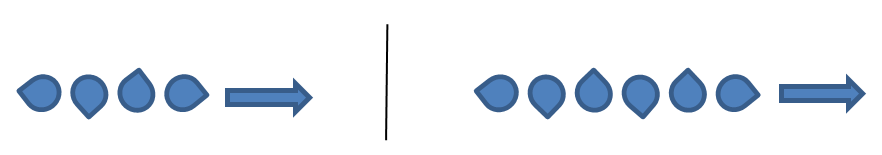
\includegraphics[width=15cm]{./img/grundlagen/formationen/Stack.png}
	\caption{Stack 4 und 6 Mann}
\end{figure}

\subsubsection{Die Kolonne}
Die Kolonne dient als Formation im offenen Gelände und ist die Standardformation für den Marsch. Hierbei muss man zwischer einer Besonderheit im \ac{TTT} der Buddy - Kolonne und der klassischen Kolonne unterscheiden. Die Buddy - Kolonne garantiert, dass beispielsweise MG-Schütze und MG-Assistent immer zusammenbleiben, zudem verringern sie die Ausfallzahl, da sich Buddys besser gegenseitig unterstützen können. Im Gegenzug ist die klassische Kolonne weniger anfällig für Sprengsätze und Beschuss. Die Abstände zwischen den Teams sollten etwa 20 m betragen.\\
\begin{minipage}[t]{1\textwidth}
	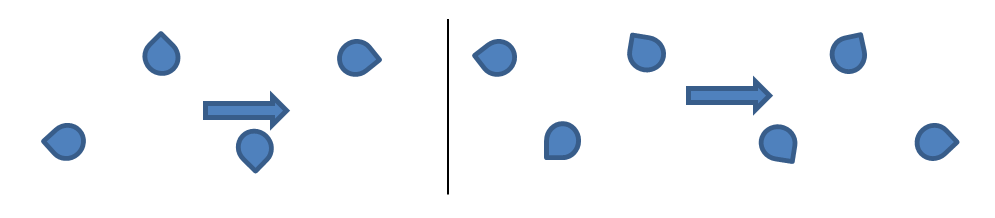
\includegraphics[width=13cm]{./img/grundlagen/formationen/Kolonne.png}
	\label{Kolonne}
\end{minipage}
\begin{minipage}[t]{1\textwidth}
	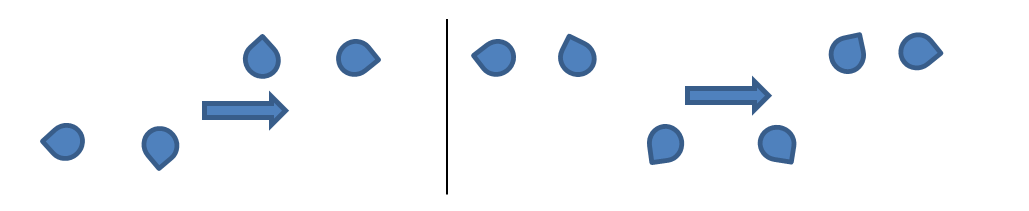
\includegraphics[width=13cm]{./img/grundlagen/formationen/Buddykolonne.png}
\end{minipage}

\subsubsection{Die Schützenkette}
Die Schützenkette ist eine Formation, die zum Bezug der Stellung, in Deckung an Mauern und -- in Ausnahmefällen! -- zum Anmarsch auf einen Feind benutzen. Sie bietet maximale Feuerkraft in vermuteter Feindrichtung, lässt jedoch die Flanken und den Rückraum ungesichert. Die Schützenkette kann effizienter gestaltet werden durch entsprechende Flanken- und Rücksicherung.\\
\begin{minipage}[t]{1\textwidth}
	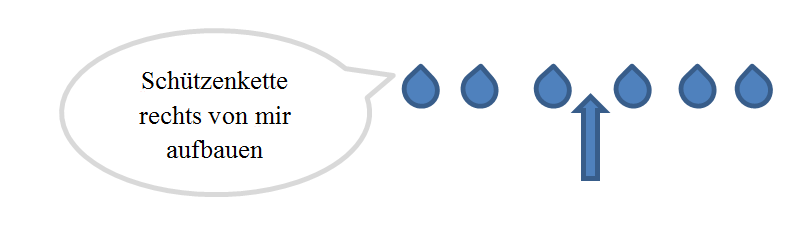
\includegraphics[width=13cm]{./img/grundlagen/formationen/Schuetzenkette1.png}
\end{minipage}
\begin{minipage}[t]{1\textwidth}
	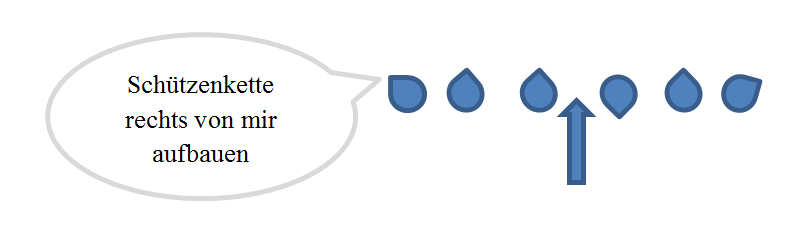
\includegraphics[width=13cm]{./img/grundlagen/formationen/Schuetzenkette2.png}
\end{minipage}